\subsubsection{Dichotomous Line Search}
The dichotomous line search is one of the most basic methods. The method locates the middle of the bracket (along x) and finds a point on either side of the middle, this gives the following two x-values at which the function must be evaluated.


\begin{flalign}
  x_a &= \frac{X_{max} - X_{min}}{2}-\epsilon \ \ \ \  \ \ \ \ x_b = \frac{X_{max} - X_{min}}{2}+\epsilon &
  \label{dichotomousXaXb}
\end{flalign}
%
\hspace{6mm} Where:\\
\begin{tabular}{ p{1cm} l l l}
& \si{x_{min}}      & is the lowest value of x in the bracket                                 & \\
& \si{x_{max}}      & is the highest value of x in the bracket                                & \\
& \si{x_a}          & is the lower value of x at which \si{f(x)} must be evaluated            & \\
& \si{x_b}          & is the upper value of x at which \si{f(x)} must be evaluated            & \\
& \si{\epsilon}     & is the small change in positive and negative direction from the middle  & \\
\end{tabular}

When the cost function, \si{f(x)} is evaluated at \si{x_a} and \si{x_b}, the two results are compared and two new possible intervals with possibility of containing the minimum can be determined as a consequence. These two intervals can be combined such that a new smaller bracket containing the minimum is found.\\
This process of reducing the range of the bracket is illustrated in \figref{dichotomousLargerAorB}. The value of \si{f(x)} is only known at the red dots, which, as shown, leaves the two possible intervals for the minimum \si{x^*}. In the case of \si{f(x_a) < f(x_b)}, in \figref{dichotomousLargerB}, the two possible intervals, \si{x_{min} < x^* < x_a} and \si{x_a < x^* < x_b}, can be combined to the new bracket \si{x_{min} < x^* < x_b}, shown in blue. This new interval is sure to contain the minimum, \si{x^*}, within \si{x_{min}} and \si{x_{max}}.\\
Said in another way, if \si{f(x_a) < f(x_b)}, \si{x^*} must be contained in \si{[x_{min},\ x_b]}, so \si{x_b = x_{max}} for the next iteration.

  \begin{figure}[H]
    \begin{minipage}{\linewidth}
      \captionsetup[subfigure]{font = footnotesize}
      \centering
      \subcaptionbox
      {
        Here \si{f(x_a) < f(x_b)} resulting in the red interval, \si{x_{min} < x^* < x_a}, and green interval, \si{x_a < x^* < x_b}, which when combined yields the new bracket, \si{[x_{min},\ x_b]}, shown in blue.
        \label{dichotomousLargerB}
      }
      {
        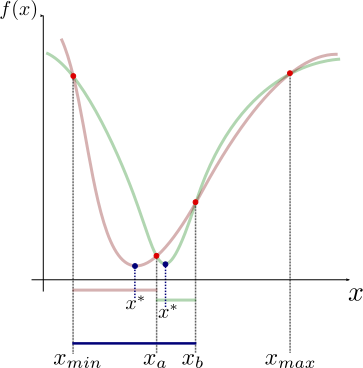
\includegraphics[scale=.6]{dichotomousLargerB}
      }\quad
      \subcaptionbox
      {
        Here \si{f(x_b) < f(x_a)} resulting in the green interval, \si{x_a < x^* < x_b}, and red interval, \si{x_b < x^* < x_{max}}, which when combined yields the new bracket, \si{[x_a,\ x_{max}]}, shown in blue.
        \label{dichotomousLargerA}
      }
      {
        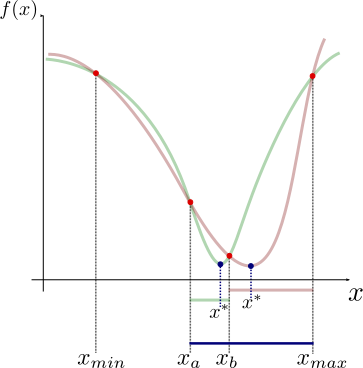
\includegraphics[scale=.6]{dichotomousLargerA}
      }
      \caption{The function, \si{f(x)}, is only evaluated at the points indicated by red dots. Two examples of how the graph of \si{f(x)} could appear is shown in green and red.}
      \label{dichotomousLargerAorB}
    \end{minipage}
  \end{figure}

In the example implementation provided in \figref{dichotomousLineSearchComprehensive} the method is demonstrated on a rough scale so that the decisions made by the algorithm are clearly seen. Red lines represent \si{x_a}, blue lines \si{x_b} and for each iteration a new \si{x_{min}} or \si{x_{max}} is selected and indicated by the dotted markings.
%
\begin{figure}[H]
	\centering
	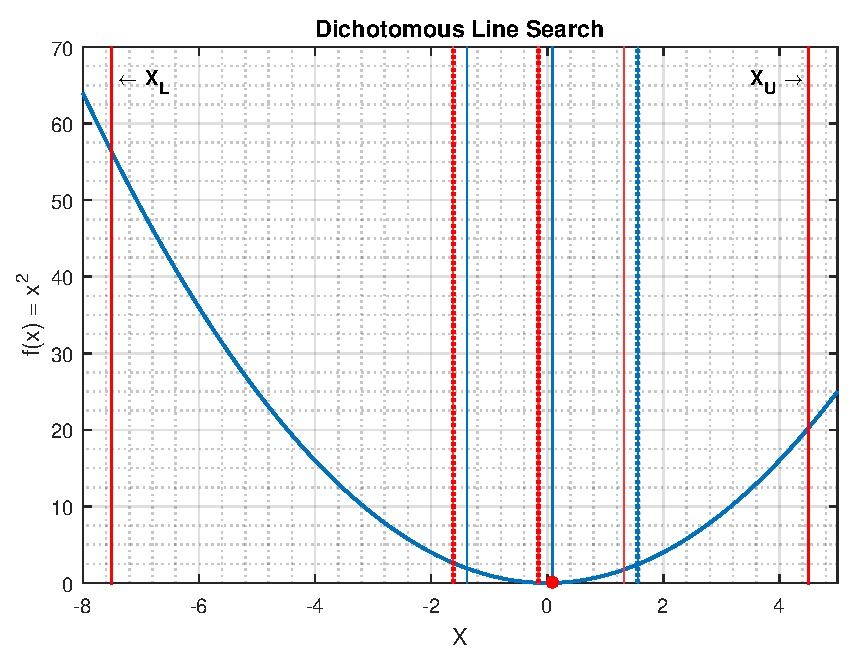
\includegraphics[width=.5\textwidth]{figures/dichotomousLineSearchComprehension.pdf}
	\caption{The bracket is marked as Xmin and Xmax, the remaining reference lines marks \si{x_a} as red and \si{x_b} as lines. The lines which are dotted are the ones selected as new Xmin, \si{x_a}, or new Xmax, \si{x_b} in each iteration.}
	\label{dichotomousLineSearchComprehensive}
\end{figure}